%%%%%%%%%%%%%%%%%%%%%%%%%%%%%%%%%%%%%%%%%%%%%%%%%%%%%%%%%%%%%%%%%%%%%%%%%%%%%%%%%%
\begin{frame}[fragile]\frametitle{}
\begin{center}
{\Large Introduction}
\end{center}
\end{frame}


%%%%%%%%%%%%%%%%%%%%%%%%%%%%%%%%%%%%%%%%%%%%%%%%%%%%%%%%%%%
\begin{frame}[fragile]\frametitle{Background}

\begin{itemize}
\item LLMs (Large Language Models) are pre-trained on large amounts of publicly available data. Sometimes having a cut-off date, say, Nov 2021.
\item How do we best augment LLMs with our own private data?
\item But how to ingest private knowledge? Many ways \ldots
\item How to use them with private data: Few shots, RAG, Fine-Tuning. 
\item Fine-tuning: adding last layer, and retraining the weights, but downsides are:
	\begin{itemize}
	\item Data preparation effort
	\item Lack of transparency
	\item May not work well
	\item High upfront cost
	\end{itemize}	
\item Most effective-middle-ground: RAG (Retriveal Augmented Generation) ie In-context learning - putting context into the prompt
\end{itemize}	


\end{frame}



%%%%%%%%%%%%%%%%%%%%%%%%%%%%%%%%%%%%%%%%%%%%%%%%%%%%%%%%%%%
\begin{frame}[fragile]\frametitle{In-context learning}

Key challenges:

\begin{itemize}
\item How to retrieve the right context for the prompt?
\item How to deal with long context? 
\item How to deal with source data that is potentially very large? (GB’s, TB’s) 
\item How to trade-off between: Accuracy, Latency, Cost
\end{itemize}	

Solution \ldots LlamaIndex

\end{frame}



%%%%%%%%%%%%%%%%%%%%%%%%%%%%%%%%%%%%%%%%%%%%%%%%%%%%%%%%%%%
\begin{frame}[fragile]\frametitle{What is LlamaIndex?}

\begin{itemize}
\item LlamaIndex, previously known as the GPT Index, is the advanced data framework for your LLM applications
\item Data Management: Data connectors (LlamaHub), Data ingestion, data parsing/slicing, data storage/indexing.
\item Data Querying: Data retrieval, response synthesis, multi-step interactions over your data.
\item LlamaIndex allows you to seamlessly integrate individual or enterprise data, including files, workplace apps, and databases, with LLM applications. 
\item Calling an LLM API is easy. Setting up a software system that can extract insights from your private data is harder.
\end{itemize}	

\end{frame}


% %%%%%%%%%%%%%%%%%%%%%%%%%%%%%%%%%%%%%%%%%%%%%%%%%%%%%%%%%%%
% \begin{frame}[fragile]\frametitle{What is LlamaIndex?}

% \begin{center}
% 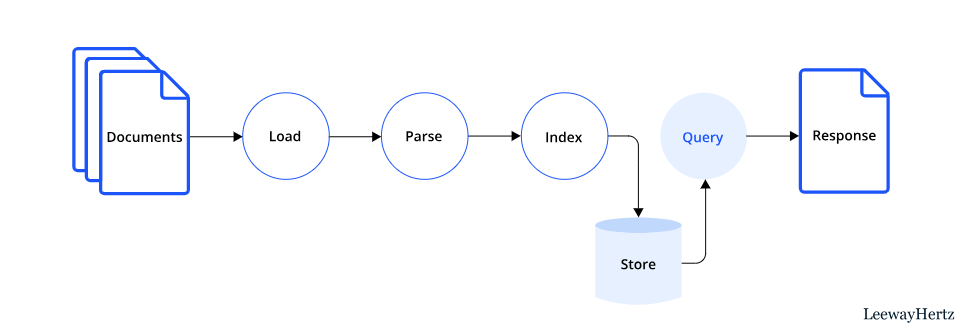
\includegraphics[width=\linewidth,keepaspectratio]{llamaindex19}

% {\tiny (Ref: What is LlamaIndex? - Leeway Hertz)}
% \end{center}
% \end{frame}

%%%%%%%%%%%%%%%%%%%%%%%%%%%%%%%%%%%%%%%%%%%%%%%%%%%%%%%%%%%
\begin{frame}[fragile]\frametitle{From Jerry Liu, co-founder, LlamaIndex?}

\begin{itemize}
\item LLMs are fantastic reasoning engines, capable of question-answering, summarization, planning, and more. They had the promise of becoming the “neural” compute unit at the core of a new age of AI-enabled software.
\item Yet, LLMs inherently have no awareness of your own data.
\item No one really knew the best practices for feeding your data into the LLM. Models had limited context windows and were expensive to finetune.
\item If we could offer a toolkit to help set up the data architecture for LLM apps, then we could enable anyone to build LLM-powered knowledge workers and transform the way that software is written over private data.
\end{itemize}	

LlamaIndex became viewed as a critical data orchestration component of the emerging LLM software landscape.

\end{frame}

%%%%%%%%%%%%%%%%%%%%%%%%%%%%%%%%%%%%%%%%%%%%%%%%%%%%%%%%%%%
\begin{frame}[fragile]\frametitle{What is Context Augmentation?}
\begin{itemize}
  \item Bridges the gap between LLMs and your private data.
  \item Ingests and makes data (PDFs, APIs, SQL, etc.) usable by LLMs.
  \item Supports full pipeline: ingest, parse, index, query.
  \item Popular use case: Retrieval-Augmented Generation (RAG).
\end{itemize}
\end{frame}



%%%%%%%%%%%%%%%%%%%%%%%%%%%%%%%%%%%%%%%%%%%%%%%%%%%%%%%%%%%
\begin{frame}[fragile]\frametitle{LlamaIndex Framework Overview}
\begin{itemize}
  \item No restriction on how LLMs are used — auto-complete, agents, etc.
  \item \textbf{Data Connectors:} Ingest from APIs, PDFs, SQL, and more.
  \item \textbf{Data Indexes:} Prepare data for fast LLM access.
  \item \textbf{Engines:} 
    \begin{itemize}
        \item Query Engines for Q\&A (e.g., RAG).
        \item Chat Engines for conversation.
    \end{itemize}
  \item \textbf{Agents:} Tool-augmented LLM knowledge workers.
  \item \textbf{Observability:} Tools to monitor, evaluate, and improve.
  \item \textbf{Workflows:} Combine all modules in flexible flows.
\end{itemize}
\end{frame}

%%%%%%%%%%%%%%%%%%%%%%%%%%%%%%%%%%%%%%%%%%%%%%%%%%%%%%%%%%%
\begin{frame}[fragile]\frametitle{Agents}
\begin{itemize}
  \item LLM-powered automated decision-makers.
  \item Use tools to interact with the world and solve tasks.
  \item Take dynamic, multi-step actions — not hardcoded sequences.
  \item Well-suited for complex, adaptive tasks.
\end{itemize}
\end{frame}

%%%%%%%%%%%%%%%%%%%%%%%%%%%%%%%%%%%%%%%%%%%%%%%%%%%%%%%%%%%
\begin{frame}[fragile]\frametitle{Workflows}
\begin{itemize}
  \item Event-driven abstractions to orchestrate LLM calls.
  \item Combine tools, agents, and logic in a structured flow.
  \item Power any agentic application in LlamaIndex.
  \item Core to building scalable LLM-based systems.
\end{itemize}
\end{frame}

%%%%%%%%%%%%%%%%%%%%%%%%%%%%%%%%%%%%%%%%%%%%%%%%%%%%%%%%%%%
\begin{frame}[fragile]\frametitle{Structured Data Extraction}
\begin{itemize}
  \item Use Pydantic extractors to define precise data schemas.
  \item LLMs fill missing pieces from unstructured sources.
  \item Enables structured outputs from PDFs, websites, etc.
  \item Crucial for automating robust workflows.
\end{itemize}
\end{frame}

%%%%%%%%%%%%%%%%%%%%%%%%%%%%%%%%%%%%%%%%%%%%%%%%%%%%%%%%%%%
\begin{frame}[fragile]\frametitle{Query Engines}
\begin{itemize}
  \item End-to-end interface for Q\&A over your data.
  \item Accepts natural language queries.
  \item Retrieves reference context and generates a response.
  \item Ideal for Retrieval-Augmented Generation (RAG).
\end{itemize}
\end{frame}

%%%%%%%%%%%%%%%%%%%%%%%%%%%%%%%%%%%%%%%%%%%%%%%%%%%%%%%%%%%
\begin{frame}[fragile]\frametitle{Chat Engines}
\begin{itemize}
  \item Built for interactive, conversational interfaces.
  \item Handle multiple back-and-forth queries with memory.
  \item Let users explore data via natural dialog.
  \item Great for copilots and customer support bots.
\end{itemize}
\end{frame}

%%%%%%%%%%%%%%%%%%%%%%%%%%%%%%%%%%%%%%%%%%%%%%%%%%%%%%%%%%%
\begin{frame}[fragile]\frametitle{Who is LlamaIndex for?}
\begin{itemize}
  \item For all levels — from beginners to experts.
  \item High-level API for quick prototyping:
  \item Low-level APIs for advanced customization.
\end{itemize}

\begin{lstlisting}[language=Python]
from llama_index import VectorStoreIndex, SimpleDirectoryReader
documents = SimpleDirectoryReader("data").load_data()
index = VectorStoreIndex.from_documents(documents)
query_engine = index.as_query_engine()
response = query_engine.query("Your question here")
\end{lstlisting}

\end{frame}

%%%%%%%%%%%%%%%%%%%%%%%%%%%%%%%%%%%%%%%%%%%%%%%%%%%%%%%%%%%
\begin{frame}[fragile]\frametitle{30 Second Quickstart}
\begin{itemize}
  \item By default, uses OpenAI gpt-3.5-turbo model for text generation and text-embedding-ada-002 for retrieval and embeddings. So, set \texttt{OPENAI\_API\_KEY} environment variable.
  \item Install the libraries
  \item Place documents in a folder named \texttt{data}.
  \item Use the 5-line starter to run a query:
  \item For advanced use, see full tutorials with remote/local models.
\end{itemize}

\begin{lstlisting}[language=Python]
pip install llama-index

---
from llama_index.core import VectorStoreIndex, SimpleDirectoryReader

documents = SimpleDirectoryReader("data").load_data()
index = VectorStoreIndex.from_documents(documents)
query_engine = index.as_query_engine()
response = query_engine.query("Some question about the data should go here")
print(response)
\end{lstlisting}
\end{frame}

%%%%%%%%%%%%%%%%%%%%%%%%%%%%%%%%%%%%%%%%%%%%%%%%%%%%%%%%%%%
\begin{frame}[fragile]\frametitle{For Open Source or Local models}
\begin{itemize}
  \item Use ollama or LM Studio for local models
  \item Use Groq (not Grok by X) API service to call Open source models
  \item Once set in Settings they are available to LlamaIndex (like global)
\end{itemize}

\begin{lstlisting}[language=Python]
from llama_index.llms.groq import Groq
from llama_index.embeddings.huggingface import HuggingFaceEmbedding
from llama_index.core import Settings

llm = Groq(model="llama3-8b-8192")
embed_model = HuggingFaceEmbedding(model_name="BAAI/bge-small-en-v1.5")
Settings.llm = llm
Settings.embed_model = embed_model
\end{lstlisting}
\end{frame}


%%%%%%%%%%%%%%%%%%%%%%%%%%%%%%%%%%%%%%%%%%%%%%%%%%%%%%%%%%%
\begin{frame}[fragile]\frametitle{LlamaCloud}
\begin{itemize}
  \item End-to-end managed service for LLM data pipelines.
  \item Handles parsing, ingestion, indexing, and retrieval.
  \item Suitable for production-grade LLM applications.
  \item Available as both hosted and self-hosted solutions.
\end{itemize}
\end{frame}

%%%%%%%%%%%%%%%%%%%%%%%%%%%%%%%%%%%%%%%%%%%%%%%%%%%%%%%%%%%
\begin{frame}[fragile]\frametitle{LlamaParse}
\begin{itemize}
  \item State-of-the-art document parser from LlamaIndex.
  \item Part of LlamaCloud or usable via self-serve API.
  \item Free plan allows parsing up to 1000 pages/day.
  \item Paid plan offers unlimited parsing with credit card.
\end{itemize}
\end{frame}


%%%%%%%%%%%%%%%%%%%%%%%%%%%%%%%%%%%%%%%%%%%%%%%%%%%%%%%%%%%
\begin{frame}[fragile]\frametitle{So, LlamaIndex: A interface between your data and LLMs }


\begin{itemize}
\item Data management + query engine
\item Goal is to make this interface fast, cheap, efficient, and performant 
\item Components:
	\begin{itemize}
	\item Data Ingestion (LlamaHub): Connect your existing data sources and data formats (API’s, PDF’s, docs, SQL, etc.)
	\item Data Structure: Store and index your data in different data structures such as lists, trees, graphs, for different use cases. 
	\item Query Interface: Feed in an input prompt and obtain a knowledge-augmented output.
	\end{itemize}	

\end{itemize}	
\end{frame}

%%%%%%%%%%%%%%%%%%%%%%%%%%%%%%%%%%%%%%%%%%%%%%%%%%%%%%%%%%%
\begin{frame}[fragile]\frametitle{Overview}
    \begin{itemize}
        \item Two key phases: data processing and querying
        \item Indexes organize document chunks (nodes) into structures
        \item Supports list, tree, and keyword table index types
        \item Customizable chunking with built-in or custom splitters
    \end{itemize}

\begin{center}
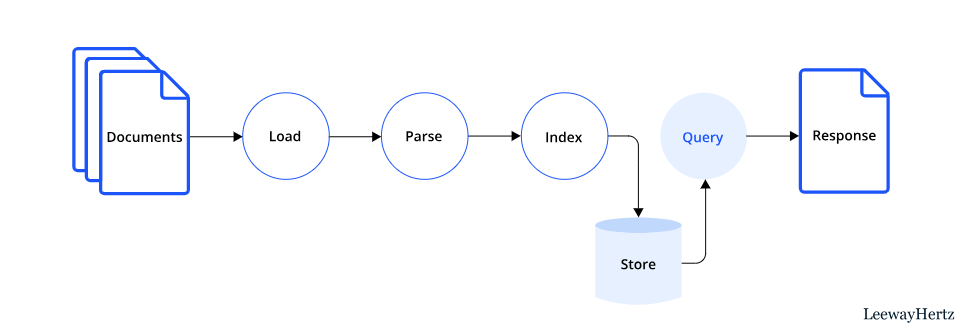
\includegraphics[width=0.8\linewidth,keepaspectratio]{llamaindex19}

{\tiny (Ref: What is LlamaIndex? - Leeway Hertz)}
\end{center}
\end{frame}

%%%%%%%%%%%%%%%%%%%%%%%%%%%%%%%%%%%%%%%%%%%%%%%%%%%%%%%%%%%
\begin{frame}[fragile]\frametitle{Index Composability}
    \begin{itemize}
        \item Indexes can be composed from other indexes, not just nodes
        \item Useful for querying across diverse data sources
        \item Tree and list indexes can combine multiple sub-indexes
        \item Summaries help guide queries to correct sub-indexes
    \end{itemize}
\end{frame}

%%%%%%%%%%%%%%%%%%%%%%%%%%%%%%%%%%%%%%%%%%%%%%%%%%%%%%%%%%%
\begin{frame}[fragile]\frametitle{Querying: List \& Vector Indexes}
    \begin{itemize}
        \item List index: sequential traversal of all nodes
        \item Prompts refined step-by-step as nodes are processed
        \item Vector index: fetches only relevant nodes via embeddings
        \item Supports external vector DBs like PineCone
    \end{itemize}
\end{frame}

%%%%%%%%%%%%%%%%%%%%%%%%%%%%%%%%%%%%%%%%%%%%%%%%%%%%%%%%%%%
\begin{frame}[fragile]\frametitle{Response Synthesis Methods}
    \begin{itemize}
        \item Create and refine: iterative response generation
        \item Tree summarize: builds a query-guided summary tree
        \item Compact: fits max nodes per prompt to reduce cost
        \item Prompts can be fully customized
    \end{itemize}
\end{frame}

%%%%%%%%%%%%%%%%%%%%%%%%%%%%%%%%%%%%%%%%%%%%%%%%%%%%%%%%%%%
\begin{frame}[fragile]\frametitle{Storage Architecture}
    \begin{itemize}
        \item Stores: document, index, and vector data
        \item Options: in-memory or MongoDB for persistence
        \item Supports external vector DBs (e.g., PineCone, Chroma)
        \item `storage\_context` aggregates all storage configs
    \end{itemize}
\end{frame}

%%%%%%%%%%%%%%%%%%%%%%%%%%%%%%%%%%%%%%%%%%%%%%%%%%%%%%%%%%%
\begin{frame}[fragile]\frametitle{What it has?}


\begin{itemize}
\item 100+ data loaders
\item 13+ vector database providers
\item Integration with observability and experimentation frameworks (e.g. prompt tracking and system tracing)
\item Integration as a ChatGPT Retrieval Plugin or with Poe
\end{itemize}	

Vision: unlocking LLM capabilities on top of your data.
\end{frame}

%%%%%%%%%%%%%%%%%%%%%%%%%%%%%%%%%%%%%%%%%%%%%%%%%%%%%%%%%%%
\begin{frame}[fragile]\frametitle{LangChain vs. LlamaIndex}

\begin{tabular}{|p{2cm}|p{4cm}|p{4cm}|}
\hline
\textbf{} & \textbf{LangChain} & \textbf{LlamaIndex} \\
\hline
\textbf{Primary Function} & 
Python library for building NLP apps with LLMs. & 
Connects LLMs to external data sources via custom indexes. \\
\hline
\textbf{Key Features} & 
Supports GPT-2/3, T5 – Tokenization, QA, summarization – Great for chatbots. & 
Links with data like Wikipedia, Stack Overflow – Topic extraction – Supports GPT-2/3/4, T5. \\
\hline
\textbf{Use Cases} & 
Chatbots, summarizing text, simple QA systems. & 
Index-based QA, topic extraction from unstructured data. \\
\hline
\end{tabular}


{\tiny (Ref: What is LlamaIndex? - Leeway Hertz)}

\end{frame}
